\documentclass{article}
\synctex=1
\def\xstacked{x̧̖̗̘̙̜̝̞̟̠̣̤̥̦̩̪̫̬̭̮̯̰̱̲̹̺̻̼͇͈͉͍̀́̂̃̄̅̆̇̈̉̊̋̌̍̎̏̑̓̔̽̾͆͝͠͡}
%\def\ttxstackedup{\sffamily x̀́̂̃̄̅̆̇̈̉̊̋̌̍̎̏̑̓̔̽̾͆͝͠͡}
%\def\ttxstackeddown{\ttfamily x̧̖̗̘̙̜̝̞̟̠̣̤̥̦̩̪̫̬̭̮̯̰̱̲̹̺̻̼͇͈͉͍}
\usepackage{polyglossia}
\setmainlanguage{english}
\setotherlanguage[variant=polytonic]{greek}
\usepackage[hidelinks,pdfa]{hyperref}
%\usepackage{xgreek}
\usepackage[default,varnothing]{fontsetup}
\usepackage{unicodefonttable,graphicx,wrapfig,xcolor,calc}
\newfontfamily\lmboldsans{lmsans10-bold.otf}
\newfontfamily\newcmaltendings[CharacterVariant=2]{NewCM10-Book.otf}
\newfontfamily\newcmaltk[CharacterVariant=1]{NewCM10-Book.otf}
\newfontfamily\newcmdlig[RawFeature=+dlig]{NewCM10-Book.otf}
%\newfontfamily\uncial{NewCMUncial10-Book.otf}
\newfontfamily\newcmgreekguillemots[CharacterVariant=4]{NewCM10-Book.otf}
\newfontfamily\newcmrussianguillemots[CharacterVariant=3]{NewCM10-Book.otf}
\newfontfamily\showtiefont[CharacterVariant=5]{NewCM10-Book.otf}
\newfontfamily\ipafont[%Renderer     = {Harfbuzz},
StylisticSet = {05},ItalicFont=NewCM10-BookItalic]{NewCM10-Book.otf}
%
%%%%%%%%%%%%%%%%%%%%%%%%%%%% Devanagari text %%%%
\newfontfamily\hinditext[%
Script=Devanagari,%
BoldFont=NewCM10Devanagari-Bold.otf,
  % Renderer=Harfbuzz% Optionally for LuaTeX
]{NewCM10Devanagari-Book.otf}
\newfontfamily\marathitext[%
Script=Devanagari,%
Language=Marathi,
  % Renderer=Harfbuzz% Optionally for LuaTeX
]{NewCM10Devanagari-Book.otf}
\newfontfamily\sanskrittext[%
Script=Devanagari,%
Language=Sanskrit,
  % Renderer=Harfbuzz% Optionally for LuaTeX
]{NewCM10Devanagari-Book.otf}
\newfontfamily\nepalitext[%
Script=Devanagari,%
Language=Nepali,
  % Renderer=Harfbuzz% Optionally for LuaTeX
]{NewCM10Devanagari-Book.otf}
\newcommand{\devanagaritext}{\marathitext}
%%%%%%%%%%%%%%%%%%%%%%%%%%%%%%%%%%%%%%%%%%%%%%%%%%

\definecolor{mygray}{gray}{.9}
\definecolor{mygrayone}{gray}{.9}
\definecolor{mygraytwo}{gray}{.8}
\definecolor{mygraythree}{gray}{.78}
\definecolor{mygrayfour}{gray}{.75}
\definecolor{mygrayfive}{gray}{.65}
\definecolor{myred}{RGB}{255,66,32}
\newfontfamily\lrgstack[Scale=2.5,Color=myred]{NewCM10-Book.otf}
\newfontfamily\lrg[Scale=4,Color=myred]{NewCM10-Book.otf}
\newfontfamily\lrgs[Scale=4,Color=myred,StylisticSet=2]{NewCMSans10-Regular.otf}
\newfontfamily\lrgsiv[Scale=4,Color=myred,StylisticSet=4]{NewCMSans10-Regular.otf}
\newfontfamily\lrgb[Scale=4,Color=myred]{NewCM10-Bold.otf}
\newfontfamily\lrgu[Scale=4,Color=myred]{NewCMUncial10-Book.otf}
\newfontfamily\grayone[Color=mygrayone,Opacity=0.7,Scale=12]{NewCM10-Book.otf}
\newfontfamily\graytwo[Color=mygraytwo,Opacity=0.7,Scale=8]{NewCM10-Book.otf}
\newfontfamily\graytwos[Color=mygraytwo,Opacity=0.7,Scale=6]{NewCM10-Book.otf}
\newfontfamily\graythree[Color=mygraythree,Opacity=0.7,Scale=12]{NewCM10-Book.otf}
\newfontfamily\grayfour[Color=mygrayfour,Opacity=0.7,Scale=10]{NewCM10-Book.otf}
\newfontfamily\grayfive[Color=mygrayfive,Opacity=0.7,Scale=12]{NewCM10-Book.otf}
\newfontfamily\ugrayone[Color=mygrayone,Opacity=0.7,Scale=9]{NewCMUncial10-Book.otf}
\newfontfamily\ugraythree[Color=mygraythree,Opacity=0.7,Scale=12]{NewCMUncial10-Book.otf}
\newfontfamily\ugrayfour[Color=mygrayfour,Opacity=0.7,Scale=10]{NewCMUncial10-Book.otf}
%
\newfontfamily\grayoneb[Color=mygrayone,Opacity=0.7,Scale=12]{NewCM10-Book.otf}
\newfontfamily\graytwob[Color=mygraytwo,Opacity=0.7,Scale=10]{NewCM10-Book.otf}
\newfontfamily\graythreeb[Color=mygraythree,Opacity=0.7,Scale=12]{NewCM10-Book.otf}
\newfontfamily\grayfourb[Color=mygrayfour,Opacity=0.7,Scale=10]{NewCM10-Book.otf}
\newfontfamily\grayfiveb[Color=mygrayfive,Opacity=0.7,Scale=12]{NewCM10-Book.otf}
\newfontfamily\devgray[Color=mygrayfive,Opacity=0.4,Scale=10,Script=Devanagari]{NewCM10Devanagari-Book.otf}
\newfontfamily\devgraytwo[Color=mygrayone,Scale=10,Script=Devanagari,Language=Marathi]{NewCM10Devanagari-Book.otf}
\newcommand\leftgrquotes{\char"201C} %{\char"2018}
\newcommand\rightgrquotes{\char"201E} %{\char"2019}
\newcommand{\acro}{\relax}
%%% Start of metadata %%%

\newtheorem{theorem}{Θεώρημα}[section]
\newtheorem{devtheorem}[theorem]{प्रमेय}

%\DeclareSymbolFont{devletters}{\encodingdefault}{NewCMMath-Regular.otf(0)}{}{}
%\ExplSyntaxOn
%\int_step_inline:nnn { "0900 } { "097F }
%{
%  \Umathcode #1 = "0 ~ \use:c{ symdevletters } ~ #1
%}
%\ExplSyntaxOff
  

\renewcommand{\arraystretch}{1.4}


\title{The New Computer Modern FontFamily\\ version 5.1}
\author{Antonis Tsolomitis}
%\address{Department of Mathematics\\ University of the Aegean\\ Karlovassi, 832\,00 Samos\\ Greece}
%\netaddress{atsol (at) aegean dot gr}
%\personalURL{https://myria.math.aegean.gr/~atsol/}
%%% End of metadata %%%
\usepackage{pstricks}
\begin{document}

%
\rput(-2,-3){\devgray ल}%
\rput(10.2,-4){\devgraytwo ल\char"093F\char"0902}%
\rput(0,0){\grayone ζ}\rput(1,-0.5){\grayfour β}
\rput(0,-5){\grayone ἆ}\rput(1,-5){\graythree ἃ}\rput(2.5,-5){\grayone ἶ}%
\rput(3.5,-5){\graythree ῗ}\rput(5,-5){\grayone ᾦ}\rput(6,-5){\graythree ᾓ}
\rput(-2,2){\scalebox{1.5}{\graythree γ}}
\rput(5,-1.5){\graytwo א}\rput(0,-10){\graytwo ש}\rput(6,-12.5){\graytwo שּׁ}
\rput(14,-14){\ugraythree Ε}
\rput(1,-14){\ugrayfour Ω}%
\rput(4.2,-19.8){\ugraythree t}
\rput(3,-21){\ugrayfour M}%
\rput(4,-15){\ugraythree D}
\rput(5,-14){\ugrayone H}
\rput(5,1.5){\grayone π}
\rput(3,1.5){\graytwo δ}
\rput(2,-11){\graytwos Ꮙ}
\rput(3,-12){\graytwo ѽ}
\rput(4,-10){\graythree Ψ}
\rput(7,-10){\grayone ɮ}
\rput(-2,-14){\graytwo ʥ}
\rput(0,-17){\ugraythree Δ}
\rput(1,-16){\grayone ξ}
\rput(5,-18){\grayfour ϋ}
\rput(9,-19){\ugrayone Β}
\rput(7,-15){\graytwo Ƅ}
\rput(10,-2){\grayfive ƴ}
\rput(-3.7,-17){\graytwo 𐅴}
\rput(6,0){\ugraythree G}
\rput(-3,-11){\graytwo ϒ}
\rput(-2,-10){\ugraythree \&}
\rput(-5,-12){\graytwo Ю}
%
\rput(0,-12){\graytwos Ꭳ}
\rput(8,-13){\graytwos Ⲍ}
\rput(9,-12){\graytwos ⲯ}
\rput(8,-15){\graytwos Ⲝ}
\rput(-2,-17){\graytwos Ꮉ}
\rput(-2.5,-20){\ugraythree @}
\rput(-1,-19){\grayfour λ}
\rput(8,-20){\graytwos Ж}
\rput(7,-21){\graytwos Ⳛ}
\rput(6,-10){\graytwos 𐅷}
\rput(7,-17){\graytwos 𐋣}
\rput(3,-18){\graytwos ⠣}
\rput(12.0,-16){\lrgstack\color{myred} \xstacked}
\rput(10,-10){{\lrgsiv Α} {\lrgs Α}}
\rput(10,-12){\lrg a A}
\rput(10,-14){\lrg  ᾃ ᾍ}
\rput(10,-16){\lrg  ⲁ Ⲁ}
\rput(10,-18){\lrgu a A}
\rput(10,-20){\lrg א אּ}
\rput(10,-22){\lrg ꭿ Ꭿ}


%
\thispagestyle{empty}
\psline[linewidth=3cm,linecolor=white](-6,-7)(17,-7)
\rput(5.5,-6.6){\color{myred}\huge The NewComputerModern FontFamily}
\rput(5.5,-7.6){\Large Antonis Tsolomitis\ \textbullet\ University of the Aegean\ \textbullet\ Department of Mathematics}
\psline[linewidth=2cm,linecolor=myred](15.9,-7)(17,-7)
\psline[linewidth=2cm,linecolor=myred](-6,-7)(-4.8,-7)



\newpage

\null\thispagestyle{empty}


%\vfill
%
%\ttxstackedup \qquad
%{\ttxstackeddown}
%
%\vfill
%

\newpage

%\end{document}

\maketitle
\tableofcontents

\section{Introduction}
The NewComputerModern FontFamily is a huge extension (``huge'' in terms of
the number of additional glyphs)
of the \verb|lm| fonts. It is not just a family adding random missing glyphs but it
adds support for several more languages and shapes needed for academic (and not only) work.
Currently it supports among others, Greek\footnote{from Claudio Beccari's Greek.},
Cyrillic\footnote{from the \texttt{cmu} package.}, Hebrew, Cherokee and
Coptic. Since it supports
diacritics stacking the number of languages that use the Latin alphabet is greatly expanded. 
Diacritics stacking is also needed for Greek for papyrological work and this is also supported.

Version 4.0 adds to the classic design of computer modern new shapes for Latin and Greek,
in particular it adds families for Medieval Latin and Uncial Greek matching in style to the
main family.

In terms of weights and sizes, all of its shapes come in Regular, Book weights
at 10 and 8 point sizes and in Bold at 10 points.

Mathematics is also supported in Regular and Book weights, currently providing
a full coverage of the Unicode Math blocks (with a few more glyphs needed for Mathematics
that Unicode has forgotten to encode).

\textit{What follows is a sequence of commands and results so as to show how to access all features
of the fonts. Character tables are also included}.


\section{How to load the fonts}
The simpler way to load the fonts is through the \verb|fontsetup| package. The command

\verb|\usepackage[default]{fontsetup}|

\noindent will load the Book weight of the NewCM family, and

\verb|\usepackage[olddefault]{fontsetup}|

\noindent will load the Regular weight.

Also notice that the fonts support the microtype package for fine typographic tuning. See the
documentation of microtype for this.

\section{The Latin alphabet}

\subsection{Ligatures and stylistic alternatives in Latin}
{\newcmaltk
The Serif font includes additional
ligatures fb ffb ffh ffj ffk fft fh fj ft fk and the same with longs instead of f
in the \textit{default} liga table (in addition to the default fi fl ffi ffl ff).
It also includes an alternative k (in the cv01 table) and
{\newcmdlig sp ch ck ct st il}
in the dlig table. Finally it also inludes} ``end'' {\newcmaltk versions for the letters
a, e, m, n and r in the cv02 table.
}
To access the alternative k load the relative font (here the Book weight) with

\verb|\setmainfont[CharacterVariant=1]{NewCM10-Book.otf}|

To load the same font with the dlig table enabled use

\verb|\setmainfont[RawFeature=+dlig]{NewCM10-Book.otf}|

and to load the font with endings variations use

\verb|\setmainfont[CharacterVariant=2]{NewCM10-Regular.otf}|

Of course the above can be mixed separating the optional arguments with comma,
or one can define a custom font say by using

\verb|\newfontfamily\myfont[<options to enable>]{NewCM10-Book.otf}|

\begin{center}
  \begin{tabular}{c|c|c|c}
    Book &   k & a e m n r & sp ch ck ct st il\\ \hline
    cv01 & {\newcmaltk k} & & \\ \hline
    cv02 & & {\newcmaltendings a e m n r} &  \\ \hline
    dlig & & & {\newcmdlig sp ch ck ct st il}
  \end{tabular}
\end{center}

\subsection{Oldstyle numbers}

Typically oldstyle numbers are available in \verb|onum| Lookup
and with the \verb|\textsc| if \verb|fontsetup| is loaded.
Also available they are with \verb|\oldstylenums|.
There are two series, one is with variable widths and one with
fixed width for use in tables. The code

\begin{verbatim}
\oldstylenums{0123456789}\addfontfeatures{Numbers=Tabular}
\textsc{0123456789}
\end{verbatim}
gives

\oldstylenums{0123456789}\addfontfeatures{Numbers=Tabular}

\textsc{0123456789}\addfontfeatures{Numbers=Proportional}

\medskip

\noindent An alternative design is also provided for the number 1 in cv06.
The code

\begin{verbatim}
\oldstylenums{0123456789}\addfontfeatures{CharacterVariant=6}
\oldstylenums{0\textcolor{red}{1}23456789}
      \addfontfeatures{CharacterVariant=6,Numbers=Tabular}
\oldstylenums{0\textcolor{red}{1}23456789}
\end{verbatim}
gives


\oldstylenums{0123456789}\addfontfeatures{CharacterVariant=6}

\oldstylenums{0\textcolor{red}{1}23456789}\addfontfeatures{CharacterVariant=6,Numbers=Tabular}

\oldstylenums{0\textcolor{red}{1}23456789}




\subsection{Old Italic}

The fonts also fully support the Old Italic Unicode block
(U10300--U1032F) in the Sans font. For example, the slots
U10307, U10310, U10312, U10314, U1031F and U1032F are
{\sffamily\char"10307\char"10310\char"10312\char"10314\char"1031F\char"1032F}.

\subsection{Diacritics Stacking}
\marginpar{\begin{center}
{\color{red}$\rightarrow$}\ \xstacked\quad{\sffamily\xstacked}\quad{\ttfamily\xstacked}\ {\color{red}$\leftarrow$}
\end{center}}
Diacritics---the full block U+0300 to U+036F---and diacritics stacking
is supported.
In the margin you can see an example of stacking on the letter ``x'' in Roman, Sans and Mono.
If you need to enter
these accents you can use the \verb|\char| command or just copy-paste from the following line
(from this pdf file or the provided source \TeX\ file):
\begin{center}
  \textit{Some} of the upper accents\\[1ex]
{\Large  ̀\quad ́\quad ̂\quad ̃\quad ̄\quad ̅\quad\quad ̆\quad ̇\quad ̈\quad ̉\quad ̊\quad ̋}\\
{\Large  ̌\quad ̍\quad ̎\quad ̏\quad ̑\quad ̓\quad ̔\quad ̽\quad ̾\quad ̚\quad ͆\quad ͝\quad ͠\quad ͡}\\
\textit{Some} of the lower accents\\
{\Large ̧\quad ̖\quad ̗\quad ̘\quad ̙\quad ̜\quad ̝\quad ̞\quad ̟\quad ̠\quad ̣\quad ̤\quad ̥\quad ̦}\\
{\Large ̩\quad ̪\quad ̫\quad ̬\quad ̭\quad ̮\quad ̯\quad ̰\quad ̱\quad ̲\quad ̹\quad ̺\quad ̻\quad ̼\quad ͇\quad ͈\quad ͉\quad ͍}
  \end{center}
  Please note that stacking is by default supported with xetex. With luatex
  you have to add the option \texttt{Renderer=Harfbuzz}, say by

  \noindent\verb|\addfontfeature{Renderer=Harfbuzz}|

Also notice that your text editor may not support stacking. The editor may show the
accents one after the other, but the pdf produced by xetex or luatex will have the accents stacked.

\subsubsection{Coloring diacritics}

If one wants to use color for diacritics, different from the color of the base character
this does not work with Xe\LaTeX\ (the commands of the \verb|color| package
break the stacking mechanism). It works though with Lua\LaTeX\ using the \verb|luacolor|
package. However, there is a problem when the base glyph and the first diacritic above
exist in the font as a precomposed character. For example, this is the case
with aacute (á) (U+00E1). Such characters are treated as one by Lua and they can not
be colorized with different colors. A work around is to place the empty character U+034F
between ``a'' and acute (U+0301). So the following minimal example
produces the result below:


\begin{verbatim}
\documentclass{article}
\usepackage[olddefault]{fontsetup}
\usepackage{luacolor}
\pagestyle{empty}
\newfontfamily{\ncmtest}[Renderer=Harfbuzz]{NewCM10-Regular.otf}
\definecolor{orange}{RGB}{255,191,0}
\definecolor{colorone}{RGB}{91,0,250}
\definecolor{colortwo}{RGB}{250,0,121}
\definecolor{colorthree}{RGB}{0,204,250}
\definecolor{colorfour}{RGB}{14,250,0}
\definecolor{colorfive}{RGB}{255,150,0}
\definecolor{colorgray}{gray}{0.8}
\newcommand{\emptydiacritic}{\char"034F}
\begin{document}
\Huge
{\ncmtest \color{colorgray}a\color{colorfour}̖\color{colortwo}̗%
\emptydiacritic\color{colorthree}́ \color{colorone}̀ \color{colorfive}̐ }
\end{document}
\end{verbatim}

\vspace{-5.5cm}


\null \hfill
\includegraphics[scale=2]{colored-diacritics.pdf}


\vspace{2cm}


\section{Greek}


The full Unicode Greek block is supported, which is
\begin{itemize}
  \item U0370--U03FF for monotonic, where missing glyphs, such as Heta (Ͱ),
    Pamphilian digamma (ͷ) etc, have been added. For example, it is now possible to write

    \centerline{βιϐλίο instead of βιβλίο.}
    
  \item U1F00--U1FFF for polytonic, and
  \item U10140--U1018F for ancient Greek numbers.
\end{itemize}
    

\begin{theorem}[Πυθαγόρειον]
Ἐν τοῖς ὀρθογω\-νί\-οις τριγώνοις τὸ ἀπὸ τῆς τὴν ὀρθὴν γωνίαν ὑπο\-τει\-νού\-σης πλευρᾶς
τετράγωνον ἴσον ἐστὶ τοῖς ἀπὸ τῶν τὴν ὀρθὴν\hspace{-1pt} γωνίαν περιεχουσῶν πλευρῶν τετραγώνοις.
\end{theorem}


Small Caps is included (in Mono font too) and all polytonic accents of Greek.
Ypogegrammeni is the default for all characters including Small Caps and prosgegrammeni
is offered as an alternative shape in the \texttt{ss01} lookup table:
\begin{center}
\begin{tabular}{c|c|c}
 &  ypogegrammeni & prosgegrammeni\\ \hline
regular &  ᾋ ᾟ ᾯ \textsc{ᾳῃῳ} & {\textprosgegrammeni{ᾋ ᾟ ᾯ \textsc{ᾳῃῳ}}}\\ \hline
sans &{\sffamily  ᾋ ᾟ ᾯ \textsc{ᾳῃῳ}} & {\sffamily{\textprosgegrammeni{ᾋ ᾟ ᾯ \textsc{ᾳῃῳ}}}}\\ \hline
mono & {\ttfamily  ᾋ ᾟ ᾯ \textsc{ᾳῃῳ}} & {\ttfamily{\textprosgegrammeni{ᾋ ᾟ ᾯ \textsc{ᾳῃῳ}}}}
\end{tabular}
\end{center}
The prosgegrammeni alternates can be accessed with 

\medskip

\verb|\textprosgegrammeni{<text>}|

\noindent or the

\verb|{\prosgegrammeni <text>}|

\medskip

\noindent of the \texttt{fontsetup} package.

\subsection{Other character variants}

Guillemots (left and right) have a different shape for Greek. For this to work
the fonts must be loaded with the cv04 character variant.

  
Compare the default guillemots: «» with Greek guillemots:
\textlang{greek}{\newcmgreekguillemots «»}. 

There is a serious problem with Unicode and the Greek anoteleia (U0387); the Greek semicolon. 
Unicode ``thinks'' that this character is the same with periodcentered (U00B7). This influences
the way keyboards are configured by several vendors such as xorg. Anoteleia
is a dot written at x-height and not at 1/2 the x-height as the periodcentered.
Although Unicode recognizes the problem\footnote{personal communication}, althought
they recognize that with their current standard you can not correctly write the Greek language,
they refuse to fix it, justifying it by saying the magical words ``backwards compatibility''
(to a \ldots{}mistake, one could add).

NewComputerModern can not allow this, as it defies the purpose of its
existence, which is to properly write every supported language. So
enabling the CharacterVariant 04 (cv04) in addition to correct
guillemots for Greek it maps periodcentered (produced by the keyboards
(in Greek Linux keyboards by AltGr+q) to proper anoteleia.

It also fixes a long standing issue with the Greek apostrophe (᾽)(U1FBD) which
is not the same with quoteright (’)(U2019). U1FBD named as ``Greek Koronis''
by Unicode is the proper character.

Another problem that has to do with
quotes inside quotes. The internal quotes in Greek should be written with
the characters quotedblleft and quotedblbase\footnote{Μανόλης Τριανταφυλλίδης, \textit{Νεοελληνική Γραμματική της δημοτικής}, Ανατύπωση της έκδοσης του \textsc{οεσβ 1941} με διορθώσεις, Θεσσαλονίκη \textsc{2002}, σελ.~\textsc{66}, ενότητα~\textsc{133}.}. For example, this is correct for Greek
\begin{center}
 {\newcmgreekguillemots  «άλφα \leftgrquotes βήτα\rightgrquotes»}
\end{center}
But the keyboards only produce quotesingle which is already mapped to apostrophe
and it is difficult to remember the names ``quotedblleft'' and ``quotedblbase''. 
So when enabling cv04 one can define the commands

\verb|\newcommand\leftgrquotes{\char"201C}| %{\char"2018}

\noindent and

\verb|\newcommand\rightgrquotes{\char"201E}| %{\char"2019}

\noindent for the rare case one needs quotes inside quotes. The \verb|fontsetup| package
does this automatically for Greek if the \verb|xgreek| package has been loaded \textit{before}
the \verb|fontsetup| package or when the language is set to Greek by, say, the Babel package.
Otherwise, for non-Greek documents with small passages of Greek,
the author may enable \verb|cv04| by creating a custom command such as

\verb|\newcommand\propergreek[CharacterVariant=4]{NewCM10-Book.otf}|


A phrase with Greek quotes inside quotes, proper anoteleia, and proper apostrophe is

\begin{center}
{\newcmgreekguillemots  «φώναζε: \leftgrquotes απ' έξω την προπαίδεια\rightgrquotes»· σαν εκδίκηση ακουγόταν\ldots}
\end{center}

\subsection{Prosodic symbols}

In Greek philology and in linguistics it is often needed to stack accent-type symbols above letters,
even if they are not vowels. Although rare in writings, it is for example valid to place dieresis
over the consonants π, τ and κ of the nasal complexes μπ, ντ, γκ
when it is necessary to show that these are pronounced, as written, voiceless, and not voiced.
For example,
\begin{center}
κομπ̈ρέσα, \quad αντιαντ̈αντ̈ικός, \quad ελεγκ̈τής
\end{center}
(see previous footnote). The fonts support this writing if a combining dieresis is placed after
the letter to receive it. The combining dieresis is the character U0308. On Linux desktops this is
easily entered pressing Alt+Control+u, release them, and type the sequence 0308 and space.

More than that, in linguistics, they need to combine several accents above Greek letters. All this
stacking of accents is supported by the fonts. For example, one can write
\begin{center}
ᾱ῏\quad ε᾿῀\quad Ἀ̆ \quad Ἆ̄ \quad ῼ᾿῀\quad ᾱ΄\quad Χ̆᾿\quad ῑ̈΄
\end{center}
by placing the combining accents from the Unicode block U0300--U0362 plus the usual Greek accents
\textit{after} the letter.
So the above was typed as
\begin{center}
{\ttfamily α ̄\hspace*{-5pt} ῏\qquad ε\hspace*{-5pt} ᾿ ῀\qquad Ἀ ̆ \quad Ἆ ̄ \qquad ῼ\hspace*{-5pt} ᾿ ῀\qquad α ̄\hspace*{-5pt} ΄\qquad Χ ̆\hspace*{-5pt} ᾿\qquad ι ̄ ̈\hspace*{-5pt} ΄}
\end{center}

\subsection{Archaic Greek writing}
The Sans Serif Regular font provides access to 6th century bce and 4th century bce Greek capitals
in ss04 and ss03 lookups. The \texttt{fontsetup} package provides commands such as\begin{center}
\verb|\textivbce{}|, \verb|\ivbce|, \verb|\textvibce{}| and \verb|\vibce|
\end{center}
%to access them if loaded
%with the \verb|[default]| or \verb|[olddefault]| option.
\begin{center}
  \begin{tabular}{c}
    6th century bce:\\ \hline
    \textvibce{ΜΗΔΕΙΣ ΑΓΕΩΜΕΤΡΗΤΟΣ ΕΙΣΙΤΩ}\\ \hline\hline
    4th century bce:\\ \hline
     \textivbce{ΜΗΔΕΙΣ ΑΓΕΩΜΕΤΡΗΤΟΣ ΕΙΣΙΤΩ}
  \end{tabular}
\end{center}
Moreover, all fonts (except Mono \&\ Math) support Ancient Greek
Numerals (the full Unicode block of Greek digits U10140--U1018E is supported),
with most symbols designed from scratch (and did not exist in C. Beccari's original fonts).
A few of the new symbols:
\begin{center}
𐅋𐅌𐅍𐅏𐅯𐅴𐆉
\end{center}
The four numerals that already existed in 
this range (that is U10144--U10147) in Beccari's fonts have been altered to a new
design matching the style of cm but also provide some Ancient Greek flair.
The new designs in Serifed and SansSerifed are:
\begin{center}
𐅄𐅅𐅆𐅇 \quad \textsf{𐅄𐅅𐅆𐅇}
\end{center}
The \texttt{fontsetup} package provides commands for all of the above symbols.
The commands follow the Unicode name of each slot (minus the ``Greek Acrophonic'').
So the Unicode slot U1014F named ``Greek Acrophonic Attic Five Staters'' can be accessed
with the command \verb|\atticfivestaters| and it gives \atticfivestaters; and the
slot u10182 named ``Greek Kyathos Base Sign'' can be accessed with the command
\verb|\greekkyathosbasesign| and it gives \greekkyathosbasesign.


\subsection{Aegean Numbers}
Aegean numbers are supported in the Sans fonts and their slots are defined in \verb|fontsetup|
package using commands of the form \verb|\aegeanXXXX| where \verb|XXXX| is the Unicode name
of the character (without spaces).
A few examples are:
\begin{center}
\aegeanseven\quad
\aegeanfivehundred\quad
\aegeanfourthousand\quad
\aegeanfiftythousand\quad
\aegeanweightbaseunit\quad
\aegeanweightfirstsubunit\quad
\aegeanweightsecondsubunit\quad
\aegeanweightthirdsubunit\quad
\aegeanweightfourthsubunit\quad
\aegeandrymeasurefirstsubunit\quad
\aegeanliquidmeasurefirstsubunit\quad
\aegeansecondsubunit\quad
\aegeanthirdsubunit
\end{center}
and the whole table of Aegean Numbers with the commands to access the glyphs
is shown on page \pageref{AegeanNumbers}.




\subsection{Support for Papyrology}
Papyrology needs to declare that a glyph is missing from the papyrus or
the papyrus is worn at this point and the papyrologist adds the missing glyph
but it is not clear from the papyrus. This is done by adding a dot below the glyph
and it is supported for all Greek glyphs in the upright fonts monotonic or polytonic:
\begin{center}
{\Large Α̣\quad Ἆ̣\quad ᾞ̣\quad ἇ̣\quad ᾦ̣\quad ῥ̣}
\end{center}
where in the source we just typed the dot below (char U0323) after the glyph.
This feature is supported for the 4th bce and 6th bce Greek in Sans:
\begin{center}
  \textvibce{\Large Γ̣Ε̣Ω̣Μ̣Ε̣Τ̣Ρ̣Ι̣Α̣}
  \quad\quad\textivbce{\Large Γ̣Ε̣Ω̣Μ̣Ε̣Τ̣Ρ̣Ι̣Α̣}
\end{center}


\subsection{Support for Chemistry}
It happens often that Greek upright characters are needed in Chemistry. People often
have trouble with this (and this is why packages such as \texttt{chemgreek} exist).
If Greek keyboard is available then it is easy; you just type in Greek, say
\texttt{β-glucan} to get ``β-glucan''.
But many writers do not have the Greek keyboard enabled, and they do not need to.
Usually they type \verb|$\beta$-glucan| but the result ``$\beta$-glucan'' is not satisfying.
One can use the ``up'' versions typing \verb|$\upbeta$-glucan| but still the result
``$\upbeta$-glucan'' looks more Math than Chemistry.
To help with this, the \texttt{fontsetup} package provides commands such as \verb|\chemAlpha|,
\verb|\chemalpha|, \verb|\chemBeta|, \verb|\chembeta|, etc. So this information essentially would
only belong to the \verb|fontsetup| documentation if it was not for kappa and rho. If we type
in Greek \texttt{κ-compound} we get ``κ-compound'' which is not satisfying, as kappa is too
cursive for this use. So the NewCM family provides an alternative kappa for this reason
and this is how \verb|\chemkappa| is defined in \verb|fontsetup|:

\verb|\newcommand{\chemkappa}{\textrm{\char"03F0}}|:
\begin{center}
  We write \verb|\chemkappa-compound| and now get ``\chemkappa-compound''.
\end{center}
(The \verb|\textrm| command in the above definition is there to make the command work
in math mode too.)
Similar is the situation for \verb|\chemrho| (\chemrho) and \verb|\chemrhoalt| (\chemrhoalt).






\section{Russian}
Russian is supported using the glyphs from the \verb|cmu| package but it has considerable
improvements (for example, the quality of the bold sans (see below)).
\begin{verse}
Я помню чудное мгновенье:\\
Передо мной явилась ты,\\
Как мимолетное виденье,\\
Как гений чистой красоты.\\
\hspace{3cm}(Пушкинъ)
\end{verse}
Again, as in Greek there is a different kind of guillemots for Russian which are available
in CharacterVariant 3 (cv03). Compare:
\begin{center}
Defaults guillemots: «» \quad Russian guillemots: {\newcmrussianguillemots «»}\quad Greek guillemots: {\newcmgreekguillemots «»}
\end{center}
Same is the situation with Russian emdash which is shorter than the default:
\begin{center}
\begin{tabular}{rl}
  Default emdash: & ---\\
  Russian emdash: & {\newcmrussianguillemots ---}
\end{tabular}
\end{center}


\section{Hebrew}
\noindent The Hebrew blocks U0590--U05FF and Hebrew Presentation forms
UFB1D--UFB4F are fully covered. and  A few letters from Hebrew: 
\begin{center}
 אבגדהושׁשּׂלּצּ
\end{center}

\section{Coptic and Epact Numbers}
\noindent The Coptic language is fully supported. This covers the Coptic blocks
in the Greek and Coptic Unicode
block (U03E2--U03EF), the full Coptic Unicode block (U2C80--U2CFF) and the Coptic Epact Numbers
(U102E0--U102FF).
A few letters from Coptic and Epact numbers follow: 
\begin{center}
ⲗⲟⲅⲟⲥ ⲛ̀ⲁⲓⲅⲩⲡⲧⲓⲟⲥ \quad 𐋡 𐋢 𐋣 𐋤 𐋥
\end{center}




\section{Cherokee}
Both Unicode blocks 
U13A0--13FF and UAB70--UABBF for Cherokee are supported. A few letters are:
%\begin{center}
  ᎣᎤᎹᏊᏐ  ꭳꭴꭷꮂꮔꮿ
%\end{center}



\section{Devanagari}

Devanagari script is supported for the serifed font in Regular (10pt/8pt), Book (10pt/8pt),
and Bold (10pt). The fonts support Hindi (as the default), Sanskrit, Marathi and Nepali Languages.
The optional arguments for the \verb|fontspec| font-selection mechanism
must include

\noindent \verb|Script=Devanagari, Language=XXXX| where \verb|XXXX|
must be replaced with one of \verb|Hindi|, \verb|Sanskrit|, \verb|Marathi|, \verb|Nepali|.
If the \verb|Language| parameter is not set then the default is \verb|Hindi|.
For Lua\LaTeX\ the parameter \verb|Renderer=Harfbuzz| must also be included.

So if say Marathi is needed as the default font document then one can use the following:
\begin{verbatim}
\usepackage{fontspec}
\setmainfont[Script=Devanagari, Language=Marathi,% 
Renderer=Harfbuzz]{NewCM10Devanagari-Book.otf}
\end{verbatim}


The Devanagari fonts were developed with the help of {\devanagaritext निरंजन} (Niranjan)
whose name appears in the copyright section of the fonts and I also thank him for
providing the samples below.


\noindent A Sanskrit sample from {\sanskrittext बृहदारण्यकोपनिषद्} (bṛhadāraṇyakopaniṣad) follows:


\begin{center}
\fbox{\begin{minipage}{9cm}
{\hinditext
ॐ पूर्णमदः पूर्णमिदं, पूर्णात्पूर्णमुदच्यते।\\
पूर्णस्य पूर्णमादाय पूर्णमेवावशिष्यते॥
}

\medskip

That\footnote{the outer world} is complete;\\
this\footnote{the inner world} too is complete.\\
From one complete comes the other. Taking out\\
one complete from the other too results in a complete.
\end{minipage}}
\end{center}


\noindent Next is a beautiful part of a poem in Marathi
by {\marathitext तुकाराम} (Tukaram) and its translation:

\medskip

\hspace*{-3cm}\begin{tabular}{l|l}
{\begin{minipage}{\widthof{\marathitext त्यांसि म्हणे जो आपुलें॥ १ ॥}}
{\marathitext
%\noindent\begin{verse} 
जें कां रंजलें गांजलें।\\
त्यांसि म्हणे जो आपुलें॥ १ ॥\\
तो चि साधु ओळखावा।\\
देव तेथें चि जाणावा॥
%\end{verse}
}
\end{minipage}}
           &
\begin{minipage}{12cm}
      %\begin{verse}
  Only the one who treats the downtrodden people equally is a sage\footnote{\ ``The wise'' of course, not the plant.}.\\
        One may sense the essence of god there.\\
      %\end{verse}
    \end{minipage}
\end{tabular}
         

\bigskip
         
Devanagari Unicode letters (range U0900--U097F) are also available as variables (letters) and
numbers in the Regular and Book Math fonts. They are available as usually in three weights
in the Math fonts so that the color is balanced when in script size (eg in exponents or indices).
For this to work a version of \verb|fontsetup| package greater or equal to 1.8 with options
\verb|default| or \verb|olddefault| loaded is needed. This is because Devanagari letters are not
Math variables in Unicode standard and hence not supported currently as such by the
unicode-math package. To show this possibility next is a theorem in Hindi (mixing with Greek):

\medskip

%प्रमेय (Πυθαγόρας - पिथागोरास)‘’
%\setmathfont[StylisticSet=4]{NewCMMath-Regular.otf}
\setmathfont[StylisticSet=4]{NewCMMath-Book.otf}
{\hinditext
\textbf{प्रमेय}\,(\textrm{Πυθαγόρας} (पिथागोरास)) अगर समकोण त्रिभुज के कर्ण की लंबाई को ‘अ’ और
अन्य दो भुजाओं की लंबाई को ‘क’ और ‘ख’ कहते हैं, तो भुजाओं की लम्बाई के वर्गों की
जोड़, कर्ण के वर्ग जितनी होती है, अर्थात्
 $अ^२=क^२+ख^२$।
}
%\setmathfont{NewCMMath-Regular.otf}
\setmathfont{NewCMMath-Book.otf}


\bigskip

However, if only Devanagari numbers are needed with the source using arabic numerals
then one can use the Stylistic Set 04 of the Math font. 
So the command

%\noindent\verb|\setmathfont[StylisticSet=4]{NewCMMath-Regular.otf}|
\noindent\verb|\setmathfont[StylisticSet=4]{NewCMMath-Regular.otf}|
with source:
\begin{verbatim}
$$\sum_{n=0}^\infty \frac1{n!}x^n=1+x+\frac{1}{2!}x^2
   +\frac1{3!}x^3+\frac1{4!}x^4+\ldots=e^x.$$
$$9!=1\cdot2\cdot3\cdot4\cdot5\cdot6\cdot7\cdot8\cdot9.$$
$$2^{2^2}$$
\end{verbatim}
will have the following effect:


%\setmathfont[StylisticSet=4]{NewCMMath-Regular.otf}
\setmathfont[StylisticSet=4]{NewCMMath-Book.otf}

$$\sum_{n=0}^\infty \frac1{n!}x^n=1+x+\frac{1}{2!}x^2+\frac1{3!}x^3+\frac1{4!}x^4+\ldots=e^x.$$
$$9!=1\cdot2\cdot3\cdot4\cdot5\cdot6\cdot7\cdot8\cdot9.$$
$$2^{2^2}$$

\noindent which when the math font is reset to use Arabic numbers with

%\noindent\verb|\setmathfont{NewCMMath-Regular.otf}| it gives:
\noindent\verb|\setmathfont{NewCMMath-Book.otf}| it gives:

%\setmathfont{NewCMMath-Regular.otf}
\setmathfont{NewCMMath-Book.otf}
$$\sum_{n=0}^\infty \frac1{n!}x^n=1+x+\frac{1}{2!}x^2+\frac1{3!}x^3+\frac1{4!}x^4+\ldots=e^x.$$
$$9!=1\cdot2\cdot3\cdot4\cdot5\cdot6\cdot7\cdot8\cdot9.$$
$$2^{2^2}$$


\section{Medieval Latin and Uncial Greek}
The family includes new shapes for medieval and uncial Greek.
The \verb|fontsetup| package provides \verb|\textuncial{<text>}| and
\verb|{\uncial text}| to use this shape. Let us write a sentence
in this shape:
\begin{center}
  \begin{minipage}{9cm}
{\uncial    The Pythagorean Theorem is one of the most important theorems in Mathematics.}\\
{\uncial    Το Πυθαγόρειο Θεώρημα είναι από τα σημαντικότερα θε\-ω\-ρή\-μα\-τα των Mαθηματικών.}
  \end{minipage}
\end{center}
\section{Braille}
Braille, both 6dot (uni2801--uni283F)
as well as 8dit (uni2840--uni28FF) patterns
are included in two versions. The Regular font provides the
characters for sighted persons (such as teachers) so they can easily see which dots are
on and which off. The Sans font contains the true Braille characters. I decided to have the
sighted version in the Regular font since a blind person does not need the real Braille pattern,
as those are produced by embossers. The Braille patterns here are meant as fonts to
typeset text mainly for sighted persons.
\begin{center}
  \begin{tabular}{c|c|c}
    & 6dot & 8dot\\ \hline
    Regular version & ⠅⠆⠇⠝⠞ & ⡂⡃⡄⡚⡛\\ \hline
    Sans version &{\sffamily ⠅⠆⠇⠝⠞} &{\sffamily ⡂⡃⡄⡚⡛}
  \end{tabular}
\end{center}

\section{Ipa symbols}

\acro{\textsc{ipa}} symbols are included and following a suggestion of Huanyu Liu
the kerning found in \texttt{tipa} package has been added here and further improved. Moreover
the letters eth, eng, beta, theta and chi
exists in \acro{\textsc{ipa}}-style in the fonts and are accessible in the ss05 lookup table since
they are in a different design from the Latin and Greek letters.
You can access this lookup table using the \verb|\textipa|
command of the fontsetup
package.
\begin{center}
  \begin{tabular}{c|c|c}
   & Non-\acro{\textsc{ipa}} & \acro{\textsc{ipa}}\\ \hline
 Regular &   ð ŋ β θ χ & \textipa{ð ŋ β θ χ}\\ \hline
 Sans & \textsf{ð ŋ β θ χ} & \textsf{\textipa{ð ŋ β θ χ}}
  \end{tabular}
\end{center}

I am grateful to {\devanagaritext निरंजन} (Niranjan) for suggesting
and testing all the \textsc{ipa} improvements that follow:


The joining of two characters such as t͜s, d͜z, k͡p, t͡ʃ etc is also supported.
The low tie is the character U035C and the upper tie is U0361. The t͜s is produced by typing the
sequence t then the low tie and then s. Similarly k͡p is produced by typing the
sequence k then the upper tie and then p. For t͜ʃ and d͜ʒ the fonts have a contextual chaining
substitution table that uses a tie which prints lower so it does not touch ʃ and ʒ.
In cases that one wants to show the tie as {\showtiefont x͜y͡z} then one needs to
enable the cv5 character variant
since the tie characters (U035C and U0361) are marks and not base glyphs.
One can do that with a command
such as

\noindent\verb|\newfontfamily{\showtie}[CharacterVariant=5]{NewCM10-Book.otf}|

There is also an older practice that such sequences are joint into a ligature. This is
not the modern way of writing but it seems than many people in the linguistics still prefer it.
The fonts support this, if one enables the \verb|lipa| table (local ipa) of the fonts.
This can be done by adding the \verb|RawFeature=+lipa| to the font specs when loading it
and it is done automatically with the commands \verb|\textoldipa{arg}| and \verb|{\oldipatext arg}|
of the \verb|fontsetup| package.

For example, \verb|\textoldipa{ts, tʃ}| produces \textoldipa{ts, tʃ}. 

All other symbols of the \verb|tipa| package are supported. Some examples are:
\begin{center}
p̚,  ˈ, ɫ, l̠, ɖ, ɟ, ʂ, e̬, k̥, m̩, t̼, t̺, etc.
\end{center}
It is worth noting that all of the above is also available in the Mono family:
\begin{ttfamily}
\begin{center}
|t͜s|t͡ʃ|\textoldipa{ts}|p̚|ˈ|ɫ|l̠|ɖ|ɟ|ʂ|e̬|k̥|m̩|t̼|t̺|
\end{center}
\end{ttfamily}

Another issue is that \textsc{ipa} used to use the Italic alternation of ``g'' even in the
upright design. This restriction was lifted in \textsc{1949} as can
be seen on page \textsc{3} in \cite{2}. % https://doi.org/10.1017\%2FS002510030000476X

Even though the normal upright shape is accepted as an
alternation, there are linguists who prefer the older
(Italic) shape ``{\ipafont g}'' and hence we are making it the default in the
stylistic set dedicated for \textsc{ipa} (ss05).

Another such case is with the ``a'' shape. It has a different
visual form in Italics ``\textit{a}'' which resembles to a distinct symbol
of \textsc{ipa} leading to a wrong transcription. In order to avoid
this confusion, we have used the slanted version ``{\itshape\ipafont a}'' of ``a'' in
ss05. The other vowel symbol (ie, ɑ (U0251)) is also
available in the fonts.



Next we give a real example of using \acro{\textsc{ipa}} symbols. The quote below is from
\textit{A course in phonetics}, {Ladefoged, Peter and Johnson, Keith}, \textsc{(2014)},
{Cengage learning}, pp.~\textsc{285--286}, and the \texttt{StylisticSet=05} has been enabled:
\begin{quote}
  Other examples of this phenomenon have also been
  mentioned.  We saw that before {\ipafont [ŋ]}, English
  does not distinguish between tense and lax vowels.
  Consequently, the vowel that occurs in, for example, sing
  has a quality between that of {\ipafont [i]} and {\ipafont
    [ɪ]}.  Similarly, there is no distinction between tense
  and lax vowels before {\ipafont [ɹ]}. The vowel in here in
  most forms of American English is also intermediate
  between {\ipafont [i]} and {\ipafont [ɪ]}. The principle
  of maximum perceptual separation also accounts for some of
  the differences between languages. French has two high
  rounded vowels, {\ipafont [u]} as in \emph{tout} {\ipafont
    [t̪u]} ``all,'' and {\ipafont [y]} as in \emph{tu}
  {\ipafont [t̪y]} ``you.''
\end{quote}




\section{Bold Sans}
\texttt{lm} fonts and \texttt{cmu} fonts do not contain a properly made
BoldSans. Their BoldSans is a stroke-extensi\-on of the Sans with rounded corners.
NewCM fixes that and provides a true BoldSans:

\hspace*{-5ex}\begin{tabular}{c|c}
  LM & NewCM\\ \hline
  & \\
  \scalebox{6.8}{\lmboldsans XΞ}&\scalebox{6.8}{\textsf{\bfseries XΞЯДЛ}}
\end{tabular}




\section{Unicode Math coverage and options}
NewCM provides
full Unicode math support, that is 
 all Mathematics Unicode Slots
 presented in \url{http://www.unicode.org/charts/}
  in both Math weights, Regular and Book. These blocks are:
\hspace*{-5em} \begin{description}
\item[Mathematical Symbols]
\ \\
Arrows (uni2190--uni21FF)\\
Supplemental Arrows-A (uni27F0--uni27FF)\\
Supplemental Arrows-B (uni2900--uni297F)\\
Supplemental Arrows-C (u1F800--u1F8FF)\\
Additional Arrows (uni2B00--uni2BFF)\\
Miscellaneous Symbols and Arrows (uni2B00--uni2BFF)
\item[Mathematical Alphanumeric Symbols] 
\ \\ (u1D400--u1D7FF)\\
     Arabic Mathematical Alphabetic Symbols\\ (u1EE00--u1EEFF)\\
     Letterlike Symbols (uni2100--uni214F)
\item[Mathematical Operators] 
\ \\ (uni2200--uni22FF)\\
    Basic operators: Plus, Factorial\\ (uni0000--uni007F)\\
             Division, Multiplication\\ (uni0080--uni00FF)\\
    Supplemental Mathematical Operators\\ (uni2A00--uni2AFF)\\
    Miscellaneous Mathematical Symbols-A\\ (uni27C0--uni27EF)\\
    Miscellaneous Mathematical Symbols-B\\ (uni2980--uni29FF)\\
    Floors and Ceilings (uni2308--uni230B)\\
    Invisible Operators (uni2061--uni2064)
  \item[Geometric Shapes (uni25A0--25FF)]
    \ \\
   Additional Shapes (uni2B00--uni2BFF)\\
   Box Drawing (uni2500--uni257F)\\
   Block Elements (uni2580--uni259F)\\
   Geometric Shapes Extended (u1F780--u1F7FF)
   \end{description}

\begin{wrapfigure}[8]{o}{0.08\textwidth}\vspace*{-1\baselineskip}
\ \\[2ex]
  \scalebox{8}{\color{gray}$\char"2BDA$}
\end{wrapfigure}
  Unfortunately, the \texttt{unicode-math} package does not
provide commands currently for the hundrends of extra glyphs that have been added
in order to fully cover the above Unicode ranges. The user can 
consult the Unicode charts at the above link and access the required 
glyph with \verb|\char"#| where \#\ is the Unicode number of the
slot the glyph belongs to. 

For example, \verb|\char"2BDA| will give the Hygeia symbol
(uni2BDA) the Rod of Asclepius as shown above (grayed and scaled $\times 8$). The glyph
that appeared in TUGboat (see \cite{1}), being more realistic will be moved to
a new font in the future with ornaments.

\subsection{Optical sizes for more glyphs}
So far the fonts provided optical sizes for 1st and 2nd order exponents for letters. This was
not true though for binary operators and some symbols commonly used in mathematics.
For example, the \verb|\perp| symbol ($\perp$) often appears in 2nd order exponents
and then it appeared very thin. Some printers could even hardly print its thin lines.
Now, such glyphs plus several binary operators, such as $+$, $-$, $\pm$, $\dotplus$ etc
are now provided in optical sizes, so that expressions such as
$$+^{+^+}\ \perp^{\perp^\perp}\ *^{*^*}\quad\frac{|P_{F^\perp}(K)|}{e^{(x+y)^*}}$$
appear on screen and print properly on printers.
Zoom or print and compare with \texttt{lat\-in\-modern-math} font:
\begin{center}
  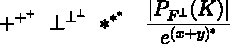
\includegraphics{opticalmathlm-cropped.pdf}
\end{center}


\subsection{Math Script}

Calligraphic letters are accessed as usual with \verb|\mathcal| producing
$$\mathcal{ABCDEFGHIJKLMNOPQRSTUVWXYZ}$$

However, mathematicians often need a second level of ``scriptness''. The fonts
provide an alternative calligraphic, a script design at StylisticSet 1. For this to work
one has to re-set the math font using

\noindent\verb|\setmathfont[StylisticSet=1]{NewCMMath-Book.otf}|

(or the Regular version). So the following code
\begin{verbatim}
$$\mathcal{ABCDEFGHIJKLMNOPQRSTUVWXYZ}$$
\setmathfont[StylisticSet=1]{NewCMMath-Book.otf}
$$\mathcal{ABCDEFGHIJKLMNOPQRSTUVWXYZ}$$
$$
\mscra\mscrb\mscrc\mscrd\mscre\mscrf\mscrg\mscrh\mscri\mscrj
\mscrk\mscrl\mscrm\mscrn\mscro\mscrp\mscrq\mscrr\mscrs\mscrt
\mscru\mscrv\mscrw\mscrx\mscry\mscrz
$$
\setmathfont{NewCMMath-Book.otf}
$$\mathcal{ABCDEFGHIJKLMNOPQRSTUVWXYZ}$$
\end{verbatim}
produces
$$\mathcal{ABCDEFGHIJKLMNOPQRSTUVWXYZ}$$\setmathfont[StylisticSet=1]{NewCMMath-Book.otf}$$\mathcal{ABCDEFGHIJKLMNOPQRSTUVWXYZ}$$
$$
\mscra\mscrb\mscrc\mscrd\mscre\mscrf\mscrg\mscrh\mscri\mscrj\mscrk\mscrl\mscrm\mscrn\mscro\mscrp\mscrq\mscrr\mscrs\mscrt\mscru\mscrv\mscrw\mscrx\mscry\mscrz
$$
\setmathfont{NewCMMath-Book.otf}$$\mathcal{ABCDEFGHIJKLMNOPQRSTUVWXYZ}$$


\subsection{Blackboard Bold}
In version 5.0 of the fonts a new NewCM blackboard bold was introduced
in the place of the \textsc{ams} blackboard
bold letters. There were many complains from Mathematicians for this choice.
I have to make a statement here: it seems that although \textsc{ams} blackboard
bold are not matching with the computer modern design the long time
Mathematicians use them had its effect. People (including myself)
got used to it and find it difficult to feel their non-matching design.
Moreover, the new design can not be metrically equivalent with the past
so there will be slight changes in the older documents if re-run.
With this in mind and the fact that the new design should be considered
``beta'', as there are characters that need improvement,
I decided bring back to default the \textsc{ams} design and keep the
new design for new documents for the StylisticSet 3. 



The \textsc{ams} blackboard bold are:
$$\mathbb{ABCDEFGHIJKLMNOPQRSTUVWXYZ}$$
$$\mathbb{abcdefghijklmnopqrstuvwxyz}$$
$$\mathbb{0123456789\ \pi\gamma\Gamma\Pi\Sigma\mitBbbD\mitBbbd\mitBbbe\mitBbbi\mitBbbj}$$

To access the new ones needs to load the math font enabling the
\verb|ss03| stylistic set using for example

\noindent\verb|\setmathfont[StylisticSet=3]{NewCMMath-Book.otf}|
Then the above blackboard bold design changes to
\setmathfont[StylisticSet=3]{NewCMMath-Book.otf}
$$\mathbb{ABCDEFGHIJKLMNOPQRSTUVWXYZ}$$
$$\mathbb{abcdefghijklmnopqrstuvwxyz}$$
$$\mathbb{0123456789\ \pi\gamma\Gamma\Pi\Sigma\mitBbbD\mitBbbd\mitBbbe\mitBbbi\mitBbbj}$$

\setmathfont{NewCMMath-Book.otf}

If using the latest \verb|fontsetup| (to be released soon)
then you can choose the NewCM blackboard bold
with the option \verb|newcmbb|.

\subsection{Upright and extensible integrals}
The Math fonts (both Regular and Book weights) include upright integrals
in the ss02 StylisticSet.
Use with

\medskip

\noindent\verb|\setmathfont[StylisticSet=2]{NewCMMath-Book.otf}|

\noindent or

\noindent\verb|\setmathfont[StylisticSet=2]{NewCMMath-Regular.otf}|

\medskip

\noindent or use the \verb|upint| option of the \texttt{fontsetup} package with
\begin{verbatim}
\usepackage[upint,default]{fontsetup}
\end{verbatim}
for the Book weight, or
\begin{verbatim}
\usepackage[upint,olddefault]{fontsetup}
\end{verbatim}
for the regular weight.


Moreover, extensible integrals are supported by the fonts but \textit{NOT} by the Unicode TeX
engines.
The following code is a trick so that extensible integrals can be
constructed using Lua\LaTeX. The result is shown at the end
of the article.
What the  code below does, is that it defines the slot uni222B (integral) as
a delimiter. And then this is extended as a delimiter with the mechanism that
the font provides.

\begin{tabular}{l|r}
  \begin{minipage}[c]{6cm}
\begin{verbatim}
\documentclass{article}
\usepackage[default]{fontsetup}
\begin{document}
$
\Uleft\Udelimiter 0 0 "222B
\begin{pmatrix}
  1\\2\\3\\4\\5\\6\\7\\8\\9
\end{pmatrix}
\Uright.
$
\end{document}
\end{verbatim}
  \end{minipage}
  &
  \begin{minipage}[c]{4cm}
\begin{center}
    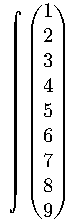
\includegraphics{integral.pdf}
\end{center}
\end{minipage}
\end{tabular}

\subsection{Additional and alternative characters in Math}
The Math fonts provide the character \verb|\varnothing| ($\varnothing$), as
an alternative to \verb|\emptyset| (a slashed zero),
through Character Variant \verb|cv01|. The \verb|fontsetup| package provides the option 
`\verb|varnothing|' to easily switch to the alternative character.

It also provides two more symbols that correspond to the commands

\medskip

  \verb|\nrightrightarrows| ($\nrightrightarrows$)

\noindent and

\verb|\nleftleftarrows| ($\nleftleftarrows$)

\medskip

\noindent
and supported by the \verb|default| and \verb|olddefault| options of the \verb|fontsetup| package.
These symbols are not in the Unicode Standard and so they are added in the
Private Area of the fonts. 


\section{The Medieval Latin and Uncial Greek glyph complement}


\displayfonttable[hex-digits=head+foot, range-end=03CE]{NewCMUncial10-Book.otf}


\section{The Aegean Numbers glyph complement}
\label{AegeanNumbers}

\begin{tabular}{|c|c||c|c|}\hline
\verb|\aegeanseparator| &\aegeanseparator&             \verb|\aegeaneighthundred| &\aegeaneighthundred\\ \hline                          
\verb|\aegeanseparatordot| &\aegeanseparatordot&       \verb|\aegeanninehundred| &\aegeanninehundred\\ \hline                            
\verb|\aegeancheckmark| &\aegeancheckmark&             \verb|\aegeanonethousand| &\aegeanonethousand\\ \hline                            
\verb|\aegeanone| &\aegeanone&                         \verb|\aegeantwothousand| &\aegeantwothousand\\ \hline                            
\verb|\aegeantwo| &\aegeantwo&                         \verb|\aegeanthreethousand| &\aegeanthreethousand\\ \hline                        
\verb|\aegeanthree| &\aegeanthree&                     \verb|\aegeanfourthousand| &\aegeanfourthousand\\ \hline                          
\verb|\aegeanfour| &\aegeanfour&                       \verb|\aegeanfivethousand| &\aegeanfivethousand\\ \hline                          
\verb|\aegeanfive| &\aegeanfive&                       \verb|\aegeansixthousand| &\aegeansixthousand\\ \hline                            
\verb|\aegeansix| &\aegeansix&                         \verb|\aegeanseventhousand| &\aegeanseventhousand\\ \hline                        
\verb|\aegeanseven| &\aegeanseven&                     \verb|\aegeaneightthousand| &\aegeaneightthousand\\ \hline                        
\verb|\aegeaneight| &\aegeaneight&                     \verb|\aegeanninethousand| &\aegeanninethousand\\ \hline                          
\verb|\aegeanine| &\aegeanine&                         \verb|\aegeantenthousand| &\aegeantenthousand\\ \hline                            
\verb|\aegeanten| &\aegeanten&                         \verb|\aegeantwentythousand| &\aegeantwentythousand\\ \hline                      
\verb|\aegeantwenty| &\aegeantwenty&                   \verb|\aegeanthirtythousand| &\aegeanthirtythousand\\ \hline                      
\verb|\aegeanthirty| &\aegeanthirty&                   \verb|\aegeanfourtythousand| &\aegeanfourtythousand\\ \hline                      
\verb|\aegeanfourty| &\aegeanfourty&                   \verb|\aegeanfiftythousand| &\aegeanfiftythousand\\ \hline                        
\verb|\aegeanfifty| &\aegeanfifty&                     \verb|\aegeansixtythousand| &\aegeansixtythousand\\ \hline                        
\verb|\aegeansixty| &\aegeansixty&                     \verb|\aegeanseventythousand| &\aegeanseventythousand\\ \hline                    
\verb|\aegeanseventy| &\aegeanseventy&                 \verb|\aegeaneightythousand| &\aegeaneightythousand\\ \hline                      
\verb|\aegeaneighty| &\aegeaneighty&                   \verb|\aegeanninetythousand| &\aegeanninetythousand\\ \hline                      
\verb|\aegeanninety| &\aegeanninety&                   \verb|\aegeanweightbaseunit| &\aegeanweightbaseunit\\ \hline                      
\verb|\aegeanonehundred| &\aegeanonehundred&           \verb|\aegeanweightfirstsubunit| &\aegeanweightfirstsubunit\\ \hline              
\verb|\aegeantwohundred| &\aegeantwohundred&           \verb|\aegeanweightsecondsubunit| &\aegeanweightsecondsubunit\\ \hline            
\verb|\aegeanthreehundred| &\aegeanthreehundred&       \verb|\aegeanweightthirdsubunit| &\aegeanweightthirdsubunit\\ \hline              
\verb|\aegeanfourhundred| &\aegeanfourhundred&         \verb|\aegeanweightfourthsubunit| &\aegeanweightfourthsubunit\\ \hline            
\verb|\aegeanfivehundred| &\aegeanfivehundred&         \verb|\aegeandrymeasurefirstsubunit| &\aegeandrymeasurefirstsubunit\\ \hline      
\verb|\aegeansixhundred| &\aegeansixhundred&           \verb|\aegeanliquidmeasurefirstsubunit| &\aegeanliquidmeasurefirstsubunit\\ \hline
\verb|\aegeansevenhundred| &\aegeansevenhundred&       \verb|\aegeansecondsubunit| &\aegeansecondsubunit\\ \hline                        
            & &                                        \verb|\aegeanthirdsubunit| &\aegeanthirdsubunit\\ \hline                          
\end{tabular}





\begin{thebibliography}{9}
\bibitem[\textsc{at}]{1} Antonis Tsolomitis, \textit{The NewComputerModern font family}, \textsc{tug}boat Vol.~\textsc{42}, No.~\textsc{1}, \textsc{2021}.
\bibitem[\textsc{ipa}rev]{2} Council actions on revisions of the \textsc{ipa}, Phonetic Representation: b) Revision of the \textsc{ipa}, Journal of the International Phonetic Association, Volume \textsc{23}, Issue \textsc{1},
  June \textsc{1993},
  pp.~\textsc{32--34}. 
\end{thebibliography}
\end{document}
